%
% File winlp2019.tex is modified based on File coling2018.tex
% 
% Contact: winlp-chairs@googlegroups.com
% if they can't help, contact: zhu2048@gmail.com & liuzy@tsinghua.edu.cn
%% Based on the style files for COLING-2018, which were in turn,
%% Based on the style files for COLING-2016, which were, in turn,
%% Based on the style files for COLING-2014, which were, in turn,
%% Based on the style files for ACL-2014, which were, in turn,
%% Based on the style files for ACL-2013, which were, in turn,
%% Based on the style files for ACL-2012, which were, in turn,
%% based on the style files for ACL-2011, which were, in turn, 
%% based on the style files for ACL-2010, which were, in turn, 
%% based on the style files for ACL-IJCNLP-2009, which were, in turn,
%% based on the style files for EACL-2009 and IJCNLP-2008...

%% Based on the style files for EACL 2006 by 
%%e.agirre@ehu.es or Sergi.Balari@uab.es
%% and that of ACL 08 by Joakim Nivre and Noah Smith

\documentclass[11pt]{article}
\usepackage{coling2018}
\usepackage{times}
\usepackage{url}
\usepackage{latexsym}
\usepackage{graphicx}
\usepackage{cleveref}
\usepackage{xcolor}
\newcommand{\sudha}[1]{\textbf{\textsf{\textcolor{blue!80!white}{\footnotesize [[Sudha: #1]]}}}}



%\setlength\titlebox{5cm}

% You can expand the titlebox if you need extra space
% to show all the authors. Please do not make the titlebox
% smaller than 5cm (the original size); we will check this
% in the camera-ready version and ask you to change it back.


\title{Controlling the Specificity of Clarification Question Generation}

\author{Sudha Rao\thanks{This research was performed when the author was still at University of Maryland, College Park.} \\
Microsoft Research, Redmond \\
{\tt Sudha.Rao@microsoft.com} \\ \And
Trista Yang Cao \\
University of Maryland, College Park \\
{\tt ycao95@cs.umd.edu} \\ \And
Hal Daum\'e III \\
University of Maryland, College Park \\
Microsoft Research, New York City\\
{\tt me@hal3.name} }


\date{}

\begin{document}
\maketitle
\begin{abstract}
Unlike comprehension-style questions, clarification questions look for some missing information in a given context. 
However, without guidance, neural models for question generation, just like other text generation tasks, lead to generic and bland questions that cannot elicit useful information. 
We propose a neural clarification question generation model with controllable level of specificity to the given context on Amazon questions dataset. 
To train the question generation model, we automatically generate the specificity labels (generic or specific) using a classifier trained on a small amount of annotated data. \sudha{this has an abrupt ending} 
%Evaluated on Amazon questions dataset, our model demonstrates controllable specificity according to both automatic metrics and human judgments.

\end{abstract}


\section{Introduction}
\label{intro}
Recent advances in neural network modeling have triggered several sequence-to-sequence learning \cite{sutskever2014sequence} based methods for question generation \cite{serban2016generating,duan2017question,du2017learning}. 
We find that training a sequence-to-sequence neural network model to generate a clarification question given a context results in over-generic questions, similar to recent findings in dialogue generation \cite{li2016deep}. 
On the other hand, we do not want a model that generates specific questions all the time. \sudha{We should maybe define what we mean by generic and specific questions before you say this.}
For instance, in Figure \ref{amazon-ex-1}, when the product description is vague, we want to first generate generic questions to fill in basic-level information.
Then when the product description is detailed, we want to generate more specific questions. \sudha{We should run this argument by Hal. I worry someone might argue that perhaps this notion of deciding when to generate specific vs generic question could/should be auto-detected by a model given a context. }
To achieve this, we take a semi-supervised approach to our problem of generating specificity controlled questions. For training data, we first construct a model that automatically predicts a question's specificity level using a small amount of annotated data (\cref{classifier}).  
Then motivated by Sennrich et al. \cite{sennrich2016controlling}, we build a question generation model that incorporates the level of specificity as an additional input signal during training\footnote{Sennrich et al. \cite{sennrich2016controlling} refer to this as side constraints.} (\cref{model}). \sudha{This should be followed by what happens during test time i.e. given a new context and a level of specificity (which is either generic or specific), the model generates question at that level of specificity.} 

\begin{figure*}[h]
	\fbox{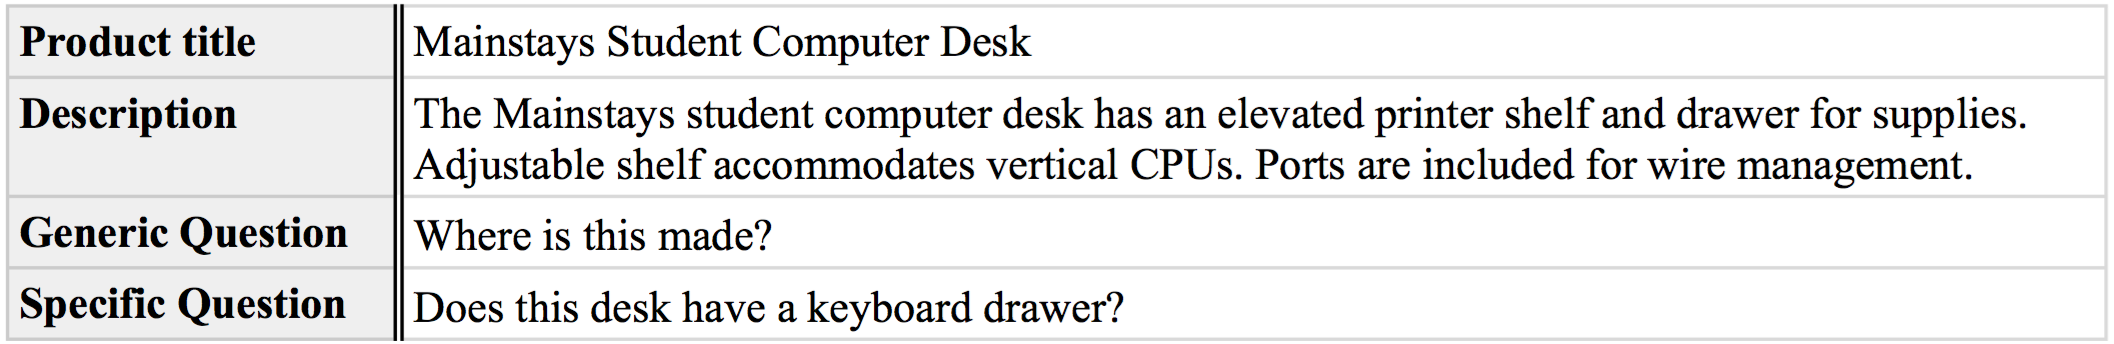
\includegraphics[width=\textwidth]{amaz-ex.png}}
    \caption{Pair of sample product description from amazon.com with a generic (left) and a specific (right) clarification question.}\label{amazon-ex-1}
\end{figure*}

\section{Related Work}
The problem of specificity level of machine-generated language \sudha{This phrase is not well-known. We should define this first.} has received sparse attention. Louis and Nenkova  \cite{louis2011automatic} first introduce a supervised binary classifier to identify specific or generic sentences \sudha{Mention that this was done under the context of summarization.}. Gao et al. \cite{Gao2019PredictingAA} then propose a supervised regression model that evaluates the level of specificity of sentence. Those works focus on identifying the specificity level of text, whereas our model focus on using the classifier to control the specificity level of question generation.

Most prior works on question generation focus on generating reading comprehension questions \cite{vanderwende2008importance}. \sudha{You should cite some recent neural network based (non-clarification) question generation models.} Comprehension questions, by definition, are answerable from the provided text. Clarification questions are not. \sudha{These two lines are exactly the same in the previous paper. Change it a bit. } Rao and Daum{\'e} III \cite{rao2019} introduce an approach for generating clarification questions using Generative Adversarial Network (GAN) \cite{goodfellow2014generative} with a sequence-to-sequence generator. \sudha{I think you should cite rao2018 first and say that they looked at ranking clarification questions. Also, I fear reviewers might point out there are some older work on clarification question generation as well. You might want to cite some of those too. I can point you to the related work in my thesis. You can borrow relevant citations from there. } 

\sudha{We can maybe combine introduction and related work to save space.}

\section{Model for Automatically Predicting Specificity Level}\label{classifier}

Given the specific/generic annotations on a subset of our training data, we want to train a machine learning model that can learn to predict the specificity level given a context and a question. Louis and Nenkova  \cite{louis2011automatic} introduce a supervised classifier for automatically predicting whether a sentence in a summary is generic or specific. We use some of the features described in their work and introduce some new features relevant to our setting to create a similar classifier that predicts the level of specificity of a question given its context. Based on these features, we train a logistic regression model to make a binary prediction (-1: generic, 1: specific) given a context and a question. We use the Support Vector Regression (SVR) model with Radial Basis Function (RBF) kernel. Gao et al. \cite{Gao2019PredictingAA}, in their work of analyzing language in social media post, claim SVR with RBF has the best performance in predicting text specificity.\\

\begin{figure*}[h]
\centering
	\fbox{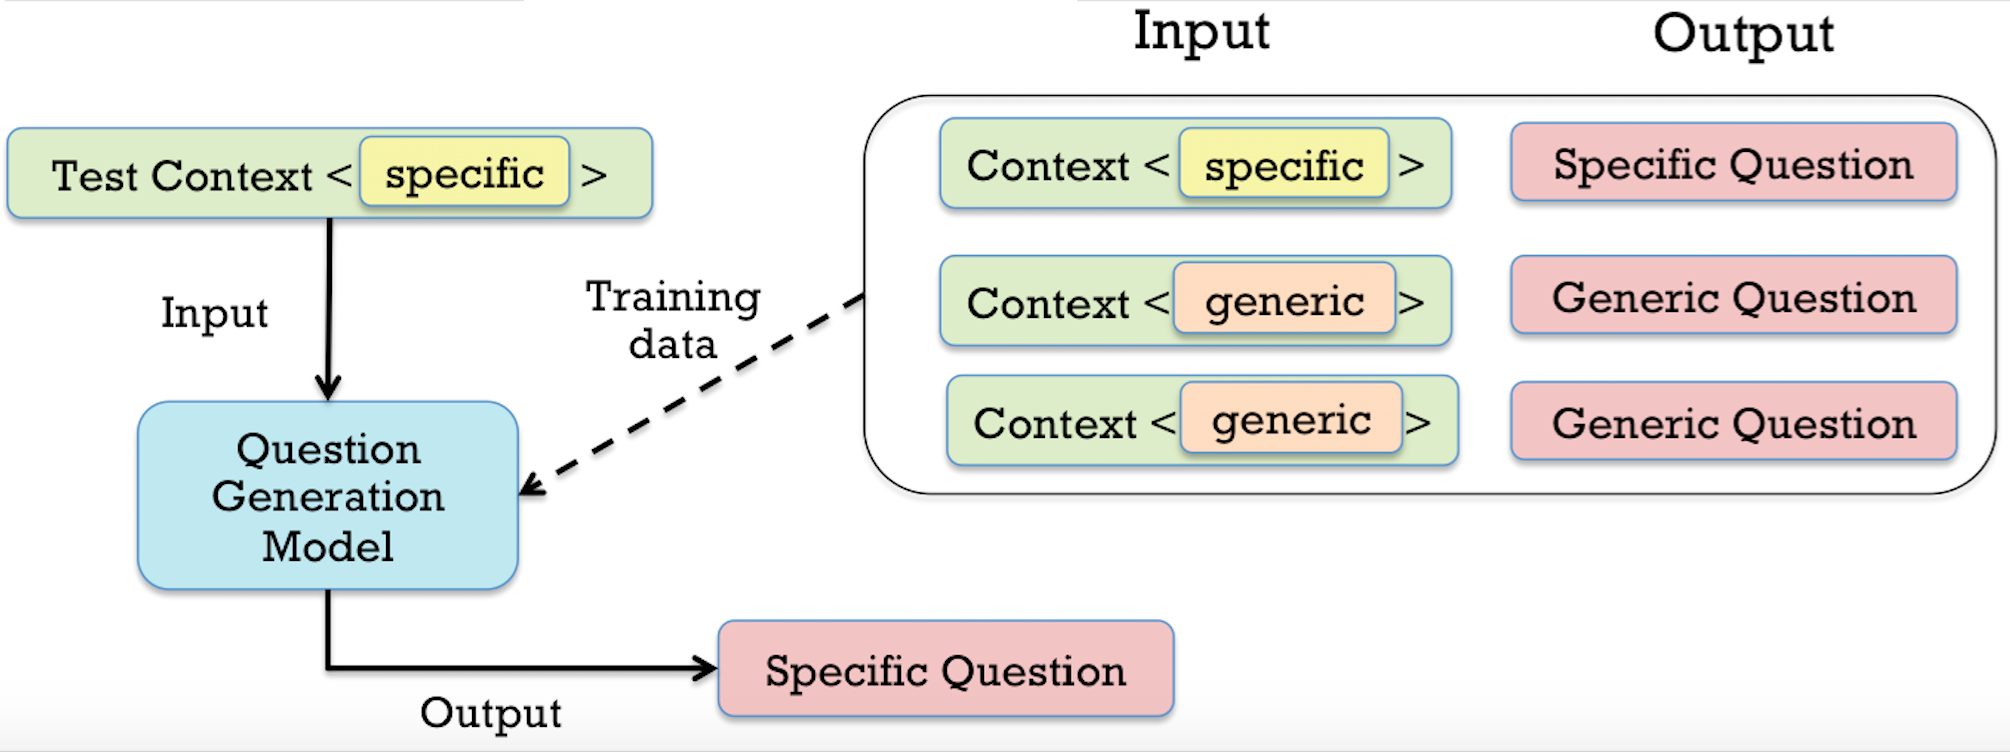
\includegraphics[scale = 0.35]{roadmap.png}}
    \caption{The behaviour of our model during test time.}\label{roadmap}
\end{figure*}
\sudha{I think we can remove this image. It will give us a lot more space. }

\section{Specificity-Controlled Question Generation Model}\label{model}
The key idea behind these sequence-to-sequence approaches is that given large amounts of input, output sequence pairs, the model learns internal representations such that at test time, given an input sequence, it generates the appropriate output sequence. 
We use the specificity classifier described in the previous section to label all the questions in the training (and tune) data with generic/specific labels. 
We use these labels to append each context with the \textit{$<$specific$>$} tag when the question paired with the context is labeled as specific and with the \textit{$<$generic$>$} tag when the question paired with the context is labeled as generic.
We train a sequence-to-sequence learning model \cite{sutskever2014sequence} on (context+specificity, question) pairs using maximum likelihood objective. 
At test time, like in figure \ref{roadmap}, we predict the specificity level of the target question using our specificity classifier and append the tag corresponding to that label to the context. \sudha{We should probably phase this differently. We should assume we are generating a question for a new context. So maybe we just say given a new context and a desirable level of specificity, we generate a question at that level of specificity. }


\section{Results/Conclusion}
We train a specificity classifier which given a context and a question can predict the level of specificity of the question to the context with $73 \%$ accuracy. 
We also conduct experiments for our specificity-controlled question generation model using Amazon questions dataset. We evaluate our results based on human evaluations. Our results have great performance on generating generic question, but not so much on generating specific ones. \sudha{`great performance' is very vague. We should be more concrete. If we do not plan to have those results by this deadline, you can just say this is work in progress. This section also requires a concluding sentence.} 

% include your own bib file like this:
%\bibliographystyle{acl}
%\bibliography{coling2018}

\bibliography{specificity_controlled_clarification}
\bibliographystyle{acl}

\end{document}
